
\chapter{Presentazione dello stage}
  \section{Descrizione del progetto di stage}
    \subsection{Prodotto}
    \subsubsection*{ERA - Enterprise Remote Assistance}
      La mission di Vision Lab Apps è il miglioramento delle condizioni di lavoro tramite l'utilizzo della tecnologia, che sviluppa strumenti \textit{hardware} e \textit{software} sempre più innovativi.\\
      ERA (Enterprise Remote Assistance) nasce dall'idea di aumentare le capacità operative del personale del settore manifatturiero tramite l'utilizzo della realtà aumentata.\\
      Nello specifico l'azienda pensa di sfruttare la potenza dei Google Glass per fornire uno strumento per permettere di:
      \begin{itemize}
        \item ricevere istruzioni sulle attività da svolgere;
        \item eseguire passaggi e procedimenti operativi;
        \item condividere informazioni;
        \item offrire supporto in tempo reale.
      \end{itemize}
      Tutto questo permette di procedere attraverso flussi di lavoro, cercando informazioni e contenuti in tempo reale.\\
      Si può inoltre tenere traccia dello svolgimento delle attività, documentandone i passaggi cruciali attraverso la registrazione di foto e video passo passo che poi potranno essere condivisi per la formazione.\\
      Si ricerca anche la funzionalità di trasmettere video in diretta, in modo da fornire assistenza in tempo reale al personale non completamente specializzato nell'attività che sta eseguendo.
    \newpage
    \subsection{Tecnologie}
    \subsubsection*{Android}
      Il prototipo dell'applicazione è stato sviluppato in Android e questo permette lo \textit{streaming} video e audio su due dispositivi in cui è installata l'applicazione.
      \begin{figure}[h]
        \centering
        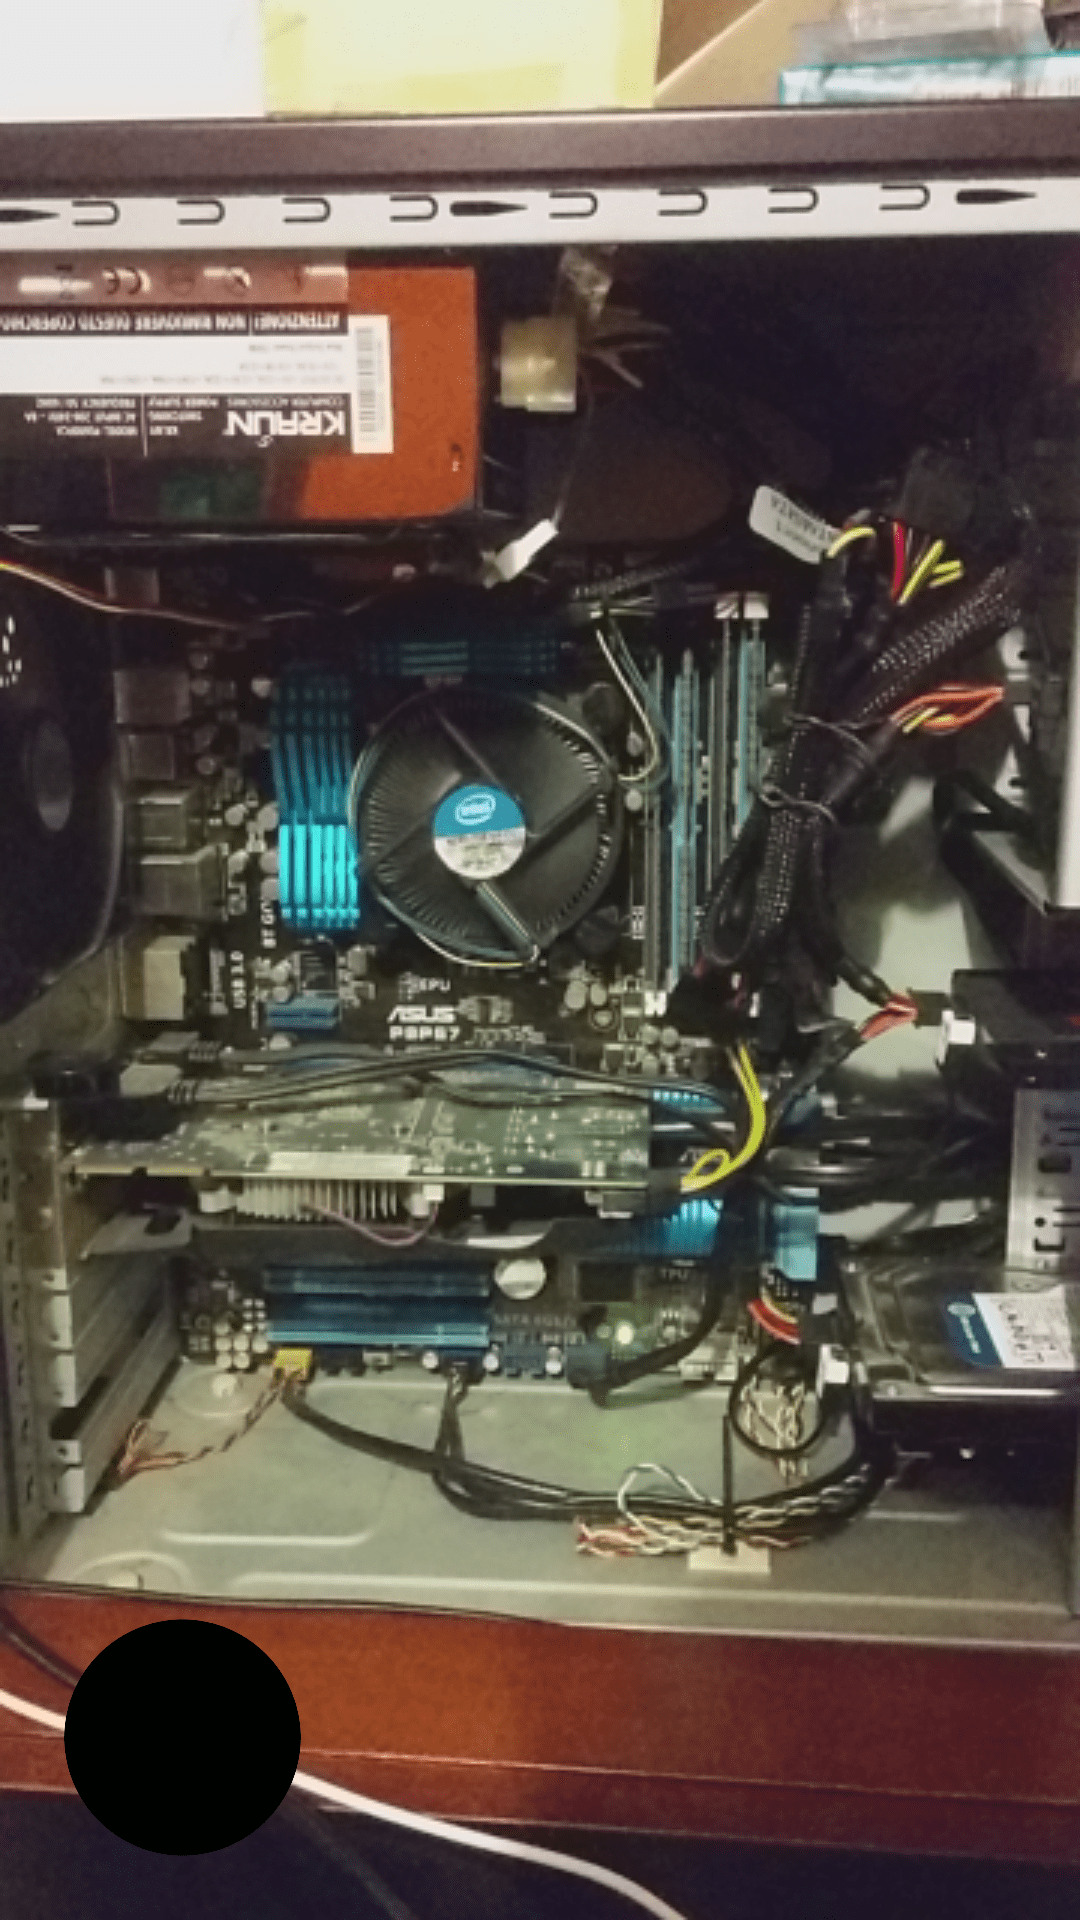
\includegraphics[width=180pt, height=320pt]{immagini/era.png}
        \caption{Streaming video su ERA}
        \label{era}
      \end{figure}
    \subsubsection*{Java}
      Per lo sviluppo del server per gestire l'autenticazione degli utenti ai vari canali, è stato sviluppato un prototipo di un'architettura client-server in Java, utilizzando il protocollo \nameref{TCP} tramite l'utilizzo di \nameref{Web}, ricercando una migliore soluzione in termini di latenza, throughput e complessità di implementazione.\\
      Lo \textit{standard} \nameref{Web} viene utilizzato per trasmettere stream di byte integrando però controlli di rete e sicurezza.\\
      Sono stati modellati, inoltre, gli utenti e nello specifico l'amministratore che può gestire i canali, controllando l'accesso ad utenti comuni.\\
      Tutto questo con una serie di controlli che permettono la gestione dei canali e dei messaggi che vengono mandati in questi stream.
    \subsubsection*{Firebase}
      In fase sperimentale è stato usato Firebase in quanto fornisce un \textit{database} e l'integrazione con dispositivi \textit{mobile}.\\
      Questo ha permesso lo sviluppo dell'applicazione Android ma anche della comunicazione con il server.
      \newpage
      \null
      \thispagestyle{empty}
      \newpage
